
\chapter{万有引力定律}
这一章我们学习万有引力定律.这个定律是牛顿在大约三百年前综合当时天文学和力学成就的基础上发现的,这个定律不仅能够说明行星和卫星的运动规律,而且能解释重力的产生和其他一些物理现像,更重要的是这个定律揭示了自然界中一种基本的相互作用力,标志着人类在认识自然的历史上迈出了重要的一步.由于万有引力定律的发现与行星运动的研究有着密切的关系,所以我们先讲一讲行星的运动.

\section{行星的运动}
在古代,人们从农牧业生产和航海的实际需要出发,就开始了对天体运动的观测和研究.我国在三千多年前的商代,根据对天体运动的观测制定了相当严密的历法.其他文明古国,如埃及、印度、巴比伦、希腊等,也在古代开始了对天体运动的研究.

对于天体的运动,历史上有过地心说和日心说两种对立的看法,地心说认为地球是宇宙的中心,它是静止不动的,太阳、月球和其他行星都围绕地球运动.日心说则相反,认为地球和其他行星是围绕太阳旋转的.日心说不符合人们的日常经验,长期内很少有人相信.

公元二世纪的希腊天文学家托勒密使地心说发展和完善起来,由于地心说能解释一些天文现像,又符合人们的日常经验,而且完全符合天主教的思想:地球是宇宙的中心,宇宙万物都是上帝创造的.所以,地心说得到教会的支持,延续了一千多年之久.但是,随着生产和航海事业的发展,天文观测资料日益丰富,人们发现托勒密地心说的理论与实际观测的资料并不完全一致,虽然对托勒密的地心说理论进行了修正,但仍不能解释某些天文现像.
\begin{figure}[H]
	\centering
	\begin{tikzpicture}[>=stealth,scale=0.8,inner sep=0pt]
		\fill[ball color=orange!50!red](0,0)circle(0.2)node[below=3mm]{\scriptsize 太阳};
		\draw[red,decoration={bumps,segment length=1.5mm,amplitude=0.7mm},decorate] (0,0) circle (0.3);
		\foreach \x/\y/\z/\w in {0.6/50/0.05,0.9/150/0.08,2.2/86/0.08,2.6/118/0.13,3.0/225/0.12}
			{
				\draw(0,0)circle(\x);
				\fill[brown](\y:\x)circle(\z);
			}
		\draw(0,0)circle(1.5);
		\fill[cyan!40](-30:1.5)circle(0.1)node[above=1mm,fill=white,text=black]{\scriptsize 地球};
		\draw(-30:1.5)circle(0.5);
		\fill[gray]([shift=(210:0.5)]-30:1.5)circle(1pt)node[left=0.5mm,text=black]{\scriptsize 月球};
		\draw[densely dashed](0,0)circle(3.3);
		\node at (86:2.2) [fill=white,below=1mm]{\scriptsize 火星};
		\node at (150:0.9)[fill=white,above=1mm]{\scriptsize 金星};
		\node at (50:0.6) [fill=white,right=1mm]{\scriptsize 水星};
		\node at (118:2.6)[fill=white,above right=1.3mm]{\scriptsize 木星};
		\node at (225:3.0)[fill=white,right=1.3mm]{\scriptsize 土星};
		\foreach \x in {1,2,...,20}
			{ \node at (rand*360:3.3) {$\ast$};}
		\draw(70:3.3)--++(70:0.3)node[above]{恒星所在球壳};
	\end{tikzpicture}
	\caption{简化了的哥白尼体系行星轨道}
\end{figure}

十六世纪,波兰天文学家哥白尼(1473—1543),经过近四十年的天文观测和研究,在古代日心说的启发下,并且利用托勒密及其后人积累的天文资料、重新提出了日心说,哥白尼日心说的主要内容是:太阳是宇宙的中心,地球和其他行星都围绕太阳公转,并且自转着(图5.1).哥白尼的学说正确地反映了行星运动的情况,可以简单明了地说明许多天文学问题,所以很快传播开了,但是日心说不符合宗教的主张,教会禁止传播哥白尼的学说,并残酷迫害接受日心说的人,用火烧死了坚持日心说的意大利人布鲁诺(1548—1600).伽利略也因为宣传日心说受到了教会的审讯和囚禁.


丹麦天文学家第谷(1546—1601)认为,要认识行星运动的规律,需要积累高度精确的观测数据、他连续二十年对行星的位置进行了精确的测量,积累了大量的数据.第谷逝世后,他的助手开普勒(1571—1630)仔细研究了第谷的观测资料,企图阐明行星运动的真实轨道,来发展和完善日心说.开普勒经过四年多的刻苦计算,先后否定了十九种设想,最后发现行星运行的真实轨道不是圆,而是椭圆,并于1609年发表了两条关于行星运动的定律:

1. \textbf{ 开普勒第一定律}:\textbf{ 所有的行星分别在大小不同的椭圆轨道上围绕太阳运动,太阳是在这些椭圆的一个焦点上}.



2. \textbf{ 开普勒第二定律}:对每个行星来说,\textbf{ 太阳和行星的联线在相等的时间内扫过相等的面积}.如图5.2所示,行星在远日点的速率最小,在近日点的速率最大.
\begin{figure}[H]
	\centering
	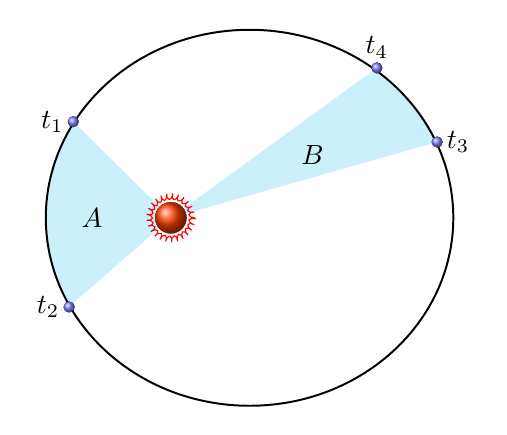
\begin{tikzpicture}[>=stealth,scale=1]
		\begin{scope}
			\path [clip](0,0)ellipse(2.6 and 2.4);
			\fill[cyan!20](-2.239,1.22)--(-1,0)--(-2.292,-1.133)to[bend left]cycle;
			\fill[cyan!20](1.617,1.904)--(-1,0)--(2.382,0.962)to[bend right]cycle;
			% \fill[cyan!20](1.434,-2.002)--(-1,0)--(0,-2.4)to[bend right]cycle;
			\fill[ball color=orange!50!red](-1,0)circle(0.2);
			\draw[red,decoration={bumps,segment length=1.5mm,amplitude=0.7mm},decorate] (-1,0) circle (0.3);
			\draw[line width =0.5mm](0,0)ellipse(2.6 and 2.4);
		\end{scope}
		\foreach \x/\y/\lc [count =\i] in {-2.239/1.22/left,-2.292/-1.133/left,2.382/0.962/right,1.617/1.904/above}
			{
				\fill[ball color=blue!50] (\x,\y)circle(2pt)node[\lc]{$t_\i$};
			}
		\node at (-2.0,0.0) {$A$};
		\node at (0.8,0.8) {$B$};
	\end{tikzpicture}
	\caption{太阳和行星的联线在相等的时间内扫过相等的面积
	}
\end{figure}

开普勒在发表了第一定律和第二定律后,进一步研究了	不同行星的运动之间的相互关系,在1619年又发表了行星运动的第三条定律,即

3. \textbf{ 开普勒第三定律}:\textbf{ 所有行星的椭圆轨道的半长轴的三次方跟公转周期的平方的比值都相等}.


由于行星的椭圆轨道都跟圆近似,在近似计算中,可以认为行星都以太阳为圆心做匀速圆周运动,在这种情况下,若用$R$代表轨道半径,$T$代表公转周期,开普勒第三定律可以用下面的公式表示:
\begin{equation}
	\frac{R^3}{T^2}=k
\end{equation}
比值$k$是一个与行星无关的恒量.

这样,开普勒提出了描述行星运动的规律,使人类的天文学知识提高了一大步.


\subsection*{练习一}
\begin{enumerate}
	\item 地球公转轨道的半径在天文学上常用来作为长度单位,叫作天文单位,用来量度太阳系内天体与太阳的距离。 (这只是个粗略的说法。在天文学中,“天文单位”有严格的定义,用符号AU表示。)已知火星公转的轨道半径是\SI{1.5}{AU},根据开普勒第三定律,火星公转的周期是多少个地球日?
	\item 开普勒行星运动定律不仅适用于行星绕太阳的运动,也适用于卫星绕行星的运动。如果一颗人造地球卫星沿椭圆轨道运动,它在离地球最近的位置(近地点)和最远的位置(远练习与应用地点),哪点的速度比较大?
	\item 有一个名叫谷神的小行星(质量$1.00\times 10^{21}~\si{kg}$),它的轨道半径是地球的2.77倍,求出它绕太阳一周需要多少年.
	\item 太阳质量大约是月球质量的$2.7\times 10^{7}$倍,太阳到地球的距离大约是月球到地球距离的$3.9\times 10^{2}$,试比较太阳和月球对地球的引力。
	\item 下表给出了太阳系九大行星平均轨道半径和周期的数值.从表中任选三个行星验证开普勒第三定律,并计算恒
	      量$k=R^3/T^2$的值.
	      \begin{table}[H]
		      \centering
		      \begin{tabularx}{0.9\textwidth}{MMM}
			      \toprule[1.5pt]
			      行星  & 平均轨道半径(m)            & 周期(s)             \\
			      \midrule
			      水星  & $5.79\times 10^{10}$ & $7.60\times 10^8$ \\
			      金星  & $1.08\times 10^{11}$ & $1.94\times 10^7$ \\
			      地球  & $1.49\times 10^{11}$ & $3.16\times 10^7$ \\
			      火星  & $2.28\times 10^{11}$ & $5.94\times 10^7$ \\
			      木星  & $7.78\times 10^{11}$ & $3.74\times 10^8$ \\
			      土星  & $1.43\times 10^{12}$ & $9.30\times 10^8$ \\
			      天王星 & $2.87\times 10^{12}$ & $2.66\times 10^9$ \\
			      海王星 & $4.50\times 10^{12}$ & $5.20\times 10^9$ \\
			      冥王星 & $5.9\times 10^{12}$  & $7.82\times 10^9$ \\
			      \bottomrule[1.5pt]
		      \end{tabularx}
	      \end{table}
\end{enumerate}
\newpage
\section{万有引力定律}
\subsection{万有引力定律}

开普勒研究了行星运动的轨道、周期和运动速率,回答了行星怎样运动的问题.然而为什么行星没有按照惯性做匀速直线运动,却围绕太阳旋转呢?十七世纪科学家们为了说明这个问题,提出了各种不同的看法.胡克等人认为,行星围绕太阳运动是因为受到了太阳对它的引力,并且猜想到引力的大小跟行星到太阳的距离的平方成反比,但是胡克没有能够从理论上证明这个猜想.

彻底解决这个问题的人是牛顿,牛顿也认为太阳对行星
的引力是行星围绕太阳运动的原因,并且运用开普勒定律和自己的力学成就,从理论上证明了引力大小跟距离的平方成反比.下面我们来看看牛顿是怎样证明的.

行星运动的轨道是椭圆,但是这些椭圆都跟圆近似,为了使问题简化,可以认为行星都以太阳为圆心做匀速圆周运动.太阳对行星的引力$F$就是行星受到的向心力.如果行星的质量是$m$,轨道半径是$R$,公转周期是$T$,根据牛顿第二定律,引
力大小$F$应该满足下面的关系:
\[F=ma_n=m\omega^2 R=\frac{4\pi^2 Rm}{T^2} \]

利用开普勒第三定律,将$T^2=R^3/k$代入上式,得
\[F=\frac{4\pi^2km}{R^2} \]

这表明,太阳对行星的引力大小$F$,跟行星与太阳的距高$R$的平方成反比,即
\[F\propto \frac{1}{R^2} \]

上面的推证不但表明太阳对行星的引力大小$F$与它们的距离$R$的平方成反比,还表明这个引力还跟行星的质量成正比,牛顿再进一步证明了,这个引力还跟太阳的质量$M$成正比,即引力跟太阳和行星的质量的乘积$Mm$成正比.把这个结果和引力与距离的平方成反比的关系结合起来,就可以得出:太阳和行星之间的引力大小,跟它们的质量的乘积成正比,跟它们的距离的平方成反比.即
\[F\propto \frac{Mm}{R^2} \]
也可以写做
\[F=G\frac{Mm}{R^2} \]
式中的$G$是个比例恒量.

牛顿还研究了卫星绕行星运动的规律,得出结论:行星和卫星之间的引力跟太阳和行星之间的引力是同一种性质的力,遵守同样的规律,即行星和卫星之间的引力大小也是跟它们的质量乘积成正比,跟它们之间的距离平方成反比.

牛顿还设想,使月球围绕地球运动的向心力和地球作用于地面上物体的重力,可能也是同一种性质的力,都是来自地球的引力,他经过计算,证明月球围绕地球运动的向心加速度大小是地面上重力加速度的1/3600,而月心和地心间的距离是地球半径的60倍,这说明地球的引力大小是跟距离的平方成反比的,从而证实了重力与天体之间的引力的确是同一性质的力.

上面的研究结果表明,太阳对行星的引力,行星对卫星的引力,以及地球对地面上物体的引力,都避循同样的规律,是同一种性质的力,于是牛顿把这种引力规律做了合理的推广,在1687年正式发表了\textbf{ 万有引力定律}:

\textbf{ 任何两个物体都是相互吸引的,引力的大小跟两个物体的质量的乘积成正比,跟它们的距离的平方成反比}.

如果用$m_1$和$m_2$表示两个物体的质量,用$r$表示它们的距离,那么万有引力定律可以用下面的公式来表示:
\begin{equation}
	F=G\frac{m_1m_2}{r^2}
\end{equation}

万有引力定律中两个物体的距离,对于相距很远可以看作是质点的物体,就是指两个质点间的距离,对于均匀的球
体,就是指两个球心间的距离.

万有引力定律的发现,是人类在认识自然规律方面取得的一个重大成果.它揭示了自然界物体间普遍存在着的一种基本相互作用——引力作用的规律,它把地球上的力学推广到天体上去,创立了将天体运动和地面物体的运动统一起来的理论,对以后物理学和天文学的发展有很大的影响.万有引力定律的发现,对人类文化历史的发展也有重要的意义.在牛顿以前,人们认为天体的运动是神秘的,隐藏着不可认识的规律.牛顿的发现,使人们解放了思想,建立了信心,相信天地间的事物和支配宇宙的自然规律都是可以认识的.
\newpage
\section{万有引力恒量的测定}
万有引力定律公式中的比例常数$G$是适用于任何两个物体的普适恒量,叫做\textbf{ 万有引力恒量}.

牛顿发现了万有引力定律,但是没有给出引力恒量$G$的数值.用实验测定$G$的大小是很不容易的,因为一般物体间的引力非常小,很难精确测定,所以在万有引力定律发现后的百余年间,一直没有测出引力恒量的准确数值,有一些科学家,为了测出物体间的引力,曾利用山峰、海岛等质量大的物体做过实验,但都没有取得令人满意的结果.

1798年,即在牛顿发现万有引力定律一百多年以后,英
国的卡文迪许(1731—1810)巧妙地利用扭秤装置,第一次在实验室里比较准确地测出了万有引力恒量的数值.

\begin{figure}[H]
	\centering
	\begin{tikzpicture}[>=stealth,scale=1.2]
		\fill[left color=gray,right color=gray,middle color=white](-0.05,0)rectangle(0.05,2.0);
		\foreach \x/\y in {2/90,1.6/75,1.1/50,0.5/20}
			{
				\draw[line width=\x pt,gray!\y](-2,-0.5)--(2,0.5);
			}
		\draw[thin](-3,-0.2)--(-3,-0.5);
		\draw[thin](-2,-0.8)--(-2,-1.2);
		\draw[thin,<->](-3,-0.4)--(-2,-1.1)node[midway,above]{$l$};
		\draw[thin](3,-0.6)--(3,-0.9);
		\draw[thin](2,0.2)--(2,-0.2);
		\draw[thin,<->](3,-0.8)--(2,-0.1)node[midway,above]{$l$};
		\draw[-latex,thick](-2,-0.5)--++(-0.5,0.35)node[above]{$F$};
		\draw[-latex,thick](2,0.5)--++(0.5,-0.35)node[right]{$F$};
		\fill[ball color=lightgray](-2,-0.5)circle(0.2)node[above=1.5mm]{$m$};
		\fill[ball color=lightgray](2,0.5)circle(0.2)node[above=1.5mm]{$m$};
		\fill[ball color=red!80!black](-3,0.2)circle(0.3)node[left=2.5mm]{$m'$};
		\fill[ball color=red!80!black](3,-0.2)circle(0.3)node[right=2.5mm]{$m'$};
		\fill[cyan!20](0.15,1.8)--(-0.15,1.5)--(-0.15,1.0)--(0.15,1.3);
		\draw[double=brown,ultra thin,double distance=0.1pt](0,2.0)--(0,3.5);
		\fill[top color=lightgray!20,bottom color=gray](-0.5,3.5)rectangle(0.5,3.75);
		\draw[thin,red,line join=round,postaction={decorate},decoration={markings,mark=between positions 0.33 and 0.9 step 0.33
					with {\arrow{>}}}](3.6,2.0)--(0,1.4)node[left=2pt,text=black]{$M$}--(4,0.6);
		\foreach \x in {-1,0,1,2}
			{
				\draw(4+0.4*\x,0.58+0.1*\x)--++(0,-0.2);
				\draw(4+0.4*\x+0.2,0.58+0.1*\x+0.05)--++(0,-0.15);
				\foreach \y in {1,2,3,4,6,7,8,9}
					{ \draw(4+0.4*\x+0.04*\y,0.58+0.1*\x+0.01*\y)--++(0,-0.10); }
			}
		\draw(5.2,0.88)--++(0,-0.2);
	\end{tikzpicture}
	\caption{卡文迪许实验示意图}
\end{figure}

如图5.3所示,卡文迪许扭秤的主要部分是一个轻而坚固的T形架,倒挂在一根石英丝的下端.T形架水平杆的两端,各装一个质量是$m$的小球,在T形架的竖直杆上装一块小平面镜$M$,可以将射来的光线反射到一根刻度尺上.实验时,把两个质量是$m'$的大球放在图中所示的位置,它们跟小球的距离相等,由于$m$受到$m'$的吸引,石英丝被扭转,石英丝扭转的角度可以从小镜$M$的反射光在刻度尺上移动的距离求出,根据扭转角度就可以算出$m$与$m'$的引力$F$.在实验过程中,为了排除气流对测量结果的影响,卡文迪许把扭秤装置放到密闭室内,在室外用望远镜进行观测.

卡文迪许经过多次实验,证明了牛顿的万有引力定律是正确的,并且测出了万有引力恒量,如果质量的单位用千克,距离的单位用米,力的单位用卡顿,卡文迪许测得的引力恒量是$6.754\times 10^{-11}~\si{N\cdot  m^2/ kg^2}$,同现代公认的$G$等于$6.67\times 10^{-11}~\si{N\cdot  m^2/ kg^2}$很接近.这个数值等于两个质量各为\SI{1}{kg}的物体,相距\SI{1}{m}时的相互吸引力.

万有引力恒量$G$的数值非常小,所以我们日常接触的那些质量不是很大的物体间的引力就非常小,我们察觉不到.例如两个质量各为\SI{100}{g}的苹果,相距\SI{10}{cm}时,它们之间的引力大小还不到一粒砂子的重量的十万分之一,两个质量各为\SI{50}{kg}的人相距\SI{1}{m}时,他们之间的引力大约等于质量为百分之一毫克的物体的重量,这相当于几百粒尘埃的重量.这样小的力我们凭感觉当然是察觉不出来的.但如果物体的质量很大,这个引力就很大,例如地球的质量是很大的,它对地面上物体的吸引力就很显著.太阳和地球之间的吸引力就更大,大约等于$3.56\times 10^{22}~\si{N}$,这样大的力如果作用在直径是\SI{9000}{kg}的钢柱两端,可以把它拉断!正是由于太阳对地球有这样大的引力,才使得地球围绕太阳转动,而不离去.

\subsection*{练习二}
\begin{enumerate}
	\item 你能说出你对地球的引力是多少吗?
	\item “我们说苹果落向地球,而不说地球向上运动碰到苹果,是因为地球的质量比苹果大得多,地球对苹果的引力比苹果对地球的引力大得多.”这种说法对吗?为什么?
	\item 两个质量都是\SI{4}{kg}的铅球,相距\SI{0.1}{m}远,它们之间的引力是多少?
	\item 用$M$表示地球的质量,$R$表示地球的半径,$T$表示月球到地球的距离.试证明,在地球引力作用下,
	      \begin{enumerate}
		      \item 地面上物体的重力加速度$g=\dfrac{GM}{R^2}$;
		      \item 月球的加速度$a_{\text{月}}=\dfrac{GM}{r^2_{\text{月地}}}$;
		      \item 已知$r_{\text{月地}}=60R$,利用(a)(b)求$a_{\text{月}}/g$;
		      \item 已知$r_{\text{月地}}=3.8\times 10^8~\si{m}$,月球绕地球运行的周期$T=27.3$天,计算月球绕地球运行的向心加速度$a_{\text{月}}$.
		      \item 已知重力加速度$g=\SI{9.8}{m/s^2}$.用(d)中算出的$a_{\text{月}}$,求$a_{\text{月}}/g$.

		            比较(c)(e)中求出的$a_{\text{月}}/g$是否相等.如果相等,则表明地球
		            对月球的引力和对地面物体的引力都遵守平方反比定律,因
		            而是同一种性质的力,牛顿就是根据这一结果证明地球对月球的引力和地面上物体所受的重力是同一种力的.
	      \end{enumerate}
\end{enumerate}

\newpage
\section{万有引力定律在天文学上的应用}
万有引力定律揭示了天体运动的规律,是研究天体运动的重要理论基础.万有引力定律的发现对天文学的发展起了很大的推动作用,取得了重大的成就.下面我们举例来说明万有引力定律在天文学上的应用.

\subsection{天体质量的计算}

应用万有引力定律可以计算天体的质量.卫星(或行星)围绕天体的运动可以
近似地看作是匀速圆周运动.假设$M$是某个天体的质量,$m$是它的一个卫星(或行星)的质量,$r$是它们之间的距离,$a_n$是卫星的向心加速度,$T$是卫星绕天体运动的周期,那么这个天体对它的卫星的引力就是卫星围绕天体运动的向心力,所以
\[G\frac{Mm}{r^2}=ma_n=\frac{4\pi^2 mr}{T^2} \]
由上式可得
\[M=\frac{4\pi^2r^3}{GT^2} \]

测出$r$和$T$,就可以算出天体质量$M$的大小.例如,地球绕太阳公转轨道的半径是$1.49\times 10^{11}~\si{m}$,公转的周期是$3.16\times 10^7~\si{s}$,所以太阳的质量为
\[\begin{split}
		M & = \frac{4\times 3.14^2\times (1.49\times 10^{11})^2}{6.67\times 10^{-11}\times (3.16\times 10^7)^2}~\si{kg} \\
		  & =1.96\times 10^{30}~\si{kg}
	\end{split} \]


同理,根据月球绕地球运转的轨道半径和周期,可以计算出地球的质量是$5. 98\times 10^{24}~\si{kg}$.

\subsection{海王星的发现}

海王星的发现是一个应用万有引力定律取得重大成就的例子.

在十八世纪,人们已经知道太阳系有七个行星,其中1781年发现的第七个行星——天王星的运动轨道,总是同根据万有引力定律计算出来的有比较大的偏离.当时有人推测,在天王星轨道外面可能还有一个未发现的行星,它对天王星的作用引起了上述的偏离.英国的亚当斯和法国的勒维烈都利用万有引力定律各自独立地计算出这个新行星的轨道.1846年9月23日晚上,德国的加勒在勒维烈指出的位置附近观察到了这个新行星.后来,天文学家就把这个太阳系的第八个行星叫做海王星.

用同样的方法,在1930年3月14日发现了太阳系的第九个行星——冥王星.

海王星、冥王星的发现进一步证明了万有引力定律的正确性,显示了它对研究天体运动的重要意义.

\subsection*{练习三}
\begin{enumerate}
	\item 应用人造地球卫星可以测定地球的质量.我国1970年4月24日发射的第一颗人造地球卫星,其周期是\SI{114}{min},它的近地点是\SI{439}{km},远地点是\SI{2384}{km},以卫星在近地点和远地点时到地心距离的平均值作为卫星轨道的平均半径,试计算地球的质量.
	\item 登月密封舱在离月球表面\SI{112}{km}的空中沿圆形轨道运行,周期是\SI{120.5}{min},月球的半径是\SI{1740}{km},根据这些数据计算月球的质量和平均密度.
\end{enumerate}
\newpage

\section{地球上物体重量的变化}
地球对物体的引力,是万有引力的一种表现,如果用$M$表示地球的质量,用$R$表示地球的半径,用$m$表示物体的质量,根据万有引力定律,物体在地球表面上受到的地球引力大小是$F=G\frac{Mm}{R^2}$.物体的重量正是由这种引力产生的.

但是物体的重量并不等于地球对物体的引力,这是因为地球在不停地自转,地球上的一切物体都随着地球自转而绕
地轴做匀速圆周运动,这就需要向心力.这个向心力的方向是垂直指向地轴的,它的大小是$f=m\omega^2r$,式中的$r$是物体距地轴的距离,$\omega$是地球自转的角速度.这个向心力来自哪里?只能来自地球对物体的引力$F$,它是引力$F$的一个分力(图5.4).\textbf{ 引力$F$的另一个分力才是物体的重力$mg$}.
\begin{figure}[H]
	\centering
	\begin{tikzpicture}[>=latex, scale=1]
		\tkzDefPoints{0/0/O, 1.414/1.414/S}
		\draw[very thick](O) circle (2);
		\draw[dashed] (O) ellipse[x radius=2, y radius=.5];
		\draw[dashed] (0,1.414) ellipse[x radius=1.414, y radius=.3];
		\draw[dashdotted](0,-2)--(0,2);
		\draw(O)--(2,0);
		\draw(0,1.414)--(S)--(O);
		\tkzDefPoints{0/1.414/S_1}
		\tkzDefPointWith[linear, K=.4](S,S_1) \tkzGetPoint{f}
		\tkzDefPointWith[linear, K=.7](S,O) \tkzGetPoint{F}
		\tkzDefPointsBy[translation = from f to S](F){F'}
		\tkzDrawSegments[very thick, ->](S,f S,F S,F')
		\tkzDrawSegments(F,f F,F')

		\tkzLabelPoints[left](O)
		\tkzLabelPoints[above left](f)
		\tkzLabelPoint[below](F'){$mg$}
		\tkzLabelPoints[below](F)
		\draw[thick](2,0) arc [start angle =0, end angle =-180, x radius=2, y radius=.5];
		\draw[thick](S) arc [start angle =0, end angle =-180, x radius=1.414, y radius=.3];


	\end{tikzpicture}


	\caption{物体的重量是地球对物体引力的一个分力}
\end{figure}

明白了这一点,我们就容易懂得,为什么同一个物体在地球上不同纬度的地方的重量不同.

在不同纬度的地方,物体做匀速圆周运动的角速度$\omega$相同,而圆周的半径$r$不同,这个半径在赤道处最大,在两极最小(等于零),由$f=m\omega^2 r$可以知道,同一个物体随着地球自转所需的向心力,在不同纬度的地方是不同的,它随着纬度的增加而减小:在赤道最大,在两极最小(等于零).

除此之外,还应该考虑到地球并不是一个理想的球体,而是一个不大规则的椭球,它的极半径是6357千米,赤道半径是\SI{6378}{km},由于极半径比赤道半径小一些,根据引力与距离平方成反比的定律,物体所受的引力在赤道上最小,随着纬度的增加而增大,在两极达到最大.

从上面的讨论可以看出,物体在赤道上所受的引力最小,需要的向心力最大;随着纬度的增加,物体受的引力增大,需要的向心力减小;在两极引力最大,需要的向心力减小到零.所以地面上同一个物体的重量,从赤道到两极是逐渐增大的.

我们知道,物体的重量等于$mg$,所以物体的重量从赤道到两极逐渐增大表示重力加速度$g$从赤道到两极逐渐增大.

同样,根据万有引力定律知道,在同一纬度,物体的重量和重力加速度$g$的数值,还随着离地面高度的增加而减小.

不过在地面附近,$g$的数值和物体的重量随纬度和离地面高度的不同而改变的量是很小的,重力加速度$g$的数值,在赤道上约为\SI{9.78}{m/s^2},在两极约为\SI{9.83}{m/s^2}.把赤道上的物体移到两极,增加的重量大约只有原来重量的千分之五.把地面上的物体升高1千米,减小的重量不超过原来重量的万分之三.所以在一般的粗略计算中,$g$和物体重量的变化可以忽略不计.

此外,物体的重量还受到地质结构的影响,例如,在埋藏着密度较大的矿石的地区,物体的重量就要比周围地区稍大一些,也就是说,这一地区的重力加速度要比周围地区稍大一
些.重力加速度的这种变化虽然很小,却是可以测出来的.根据这种重力异常现像,可以探测地下的矿床,这种探矿方法叫
做重力探矿,是一种很重要的探矿方法.
\newpage
\section{人造地球卫星}

在第四章平抛运动里我们讨论过,在地面上高度是$h$的一点,以初速度$v$向水平方向抛射的物体,将沿着抛物线轨道
落在地平面上,在讨论这种运动时,我们认为地球表面是一个理想的平面,重力加速度的方向和大小都是恒定的,在初速度比较小,物体的射程不大时,这样处理是正确的.由于地球实际上是一个球体,如果物体的初速度比较大、射程比较远,上述处理就不准确了,当抛出的物体沿曲线轨道下落时,地面也沿着球面向下弯曲,重力的方向也跟着改变了,牛顿在研究天空中卫星的运动和地面附近的落体运动的关系时,讨论过这个问题,图5.5是在他的著作里画的一幅原理图.图中表示出从高山上用不同的水平速度抛出的物体轨迹.物体的速度越大,落地点离山脚越远.当速度足够大时,物体将环绕地球运转,成为一个人造地球卫星.
\begin{figure}[H]
	\centering
	\begin{tikzpicture}[>=stealth,scale=1.2]
		\draw(0,0)circle(2);
		\draw(0,2.0)arc(90:-90:1.6 and 1.75);
		\draw(0,2.0)arc(90:0:1.4 and 1.75);
		\draw(0,2.0)arc(90:0:1.2 and 1.75);
		\fill[brown](95:1.5)--(92:1.7)--(90:2.0)--(89:1.85)--(87:1.80)--(84:1.5);
		\begin{scope}
			\path [clip] (0,0) circle(1.5);
			\node[fill=brown] {\textcolor{cyan!20}{\resizebox{4.5cm}{!}{\faGlobeAsia}}};
		\end{scope}
	\end{tikzpicture}
	\caption{牛顿说明人造地球卫星原理的草图}
\end{figure}

\subsection{宇宙速度}

既然物体的速度足够大时,物体将环绕地球运转,成为一个人造地球卫星,那么物体的速度究竞要多大才行呢?计算人造地球卫星的速度,需要运用牛顿运动定律和万有引力定律.设质量是$m$的卫星在离地心$r$的高空环绕地球运转,它的速度是$v$.地球的质量是$M$,卫星做匀速圆周运动所需要的向心力是地球对它的引力,即
\[G\frac{Mm}{r^2}=m\frac{v^2}{r},\qquad v=\sqrt{\frac{GM}{r}} \]

从上式可以看出,$r$越大,即卫星离地面越高,它环绕地球运动的速度$v$越小.对于靠近地面运转的卫星,可以认为$r$差不多等于地球的半径$R_{\text{地}}$.地球对卫星的引力差不多等于
卫星的重量$mg$.从
\[mg=m\frac{v^2}{R_{\text{地}}} \]
可以得到
\[v=\sqrt{gR_{\text{地}}}\]
将$g=\SI{0.0098}{km/s^2}$和$R_{\text{地}}=6400$千米代入上式,得到$v=\SI{7.9}{km/s}$,这就是人造地球卫星在地面附近环绕地球做匀速圆周运动必须具有的速度,叫做\textbf{ 第一宇宙速度},也叫\textbf{ 环绕速度}.

如果人造地球卫星进入轨道的水平速度大于\SI{7.9}{km/s},而小于\SI{11.2}{km/s},它绕地球运动的轨迹就不是圆,而是椭圆(图5.6).当物体的速度等于或大于\SI{11.2}{km/s}的
时候,物体就可以挣脱地球引力的束缚,成为绕太阳运动的人造行星,或飞到其他行星上去,所以\SI{11.2}{km/s}这个速度叫做\textbf{ 第二宇宙速度},也叫\textbf{ 脱离速度}.
\begin{figure}[H]
	\centering
	\begin{tikzpicture}[>=stealth,scale=1.0]
		\useasboundingbox(-7.8,4.8)rectangle(2.0,-3.4);
		\begin{scope}[rotate=-30]
			\draw(0,0)circle(1.2);
			\draw[thin,dashed] (-7,0)--(2,0);
			\draw(-1.3,0)ellipse(2.6 and 2.0);
			\draw(-2.6,0)ellipse(3.9 and 2.5);
			\draw(-2.6,4)..controls(0,2.5)and(1.3,1.5)..(1.3,0)..controls(1.3,-1.5)and(0,-2.5)..(-2.6,-4);
			\draw(-2.6,5.2)..controls(0,3)and(1.3,1.5)..(1.3,0)..controls(1.3,-1.5)and(0,-3)..(-2.6,-5.2);
			\node at (-6.7,0)[below left]{椭圆};
			\node at (-4.7,2.1)[above,rotate=0]{$\SI{7.9}{km/s}<v<\SI{11.2}{km/s}$};
			\node at (135:1.2)[above,rotate=0]{$v=\SI{7.9}{km/s}$};
			\node at (-2.6,-4)[left]{$v=\SI{11.2}{km/s}$};
			\node at (-2.6,-5.2)[left]{$v=\SI{16.7}{km/s}$};
			\begin{scope}
				\path [clip] (0,0) circle(1.0);
				\node[fill=brown] {\textcolor{cyan!20}{\resizebox{2.5cm}{!}{\faGlobeAmericas}}};
			\end{scope}
		\end{scope}
	\end{tikzpicture}
	\caption{三个宇宙速度}
\end{figure}

达到第二宇宙速度的物体还受着太阳引力的束缚,要想
使物体挣脱太阳的束缚,飞到太阳系以外的宇宙空间去,必须使它的速度等于或大于\SI{16.7}{km/s},这个速度叫做 \textbf{ 第三宇宙速度},也叫\textbf{ 逃逸速度}.

三个宇宙速度的值都很大,要得到这样大的速度需要利用多级火箭.

\subsection{人造地球卫星中的超重和失重}

在第三章里,我们已经学过超重和失重现像,现在我们再来谈谈人造卫星中的超重和失重.

卫星发射时在加速升高的过程中,以及卫星再进入大气层向下降落的减速过程中,都有一个向上的加速度,这时就发生超重现像,这时宇宙飞行员的身体像是被一个很大的压力压住,动弹不得,想举起手来,也很困难,超重对人的生理机能也有影响,宇宙飞行员选择合适的姿态,能够在100秒钟内承受等于体重九到十倍的超重,但是超重超出一定限度就有生命危险了.

人造卫星进入轨道以后,有一个向下的加速度,因而发生失重现像,这个向下的加速度就是卫星绕地球做圆周运动的向心加速度,与升降机的情况不同的是,这个向下的加速度即向心加速度不是改变人造卫屋的速度的大小,而是不断改变人造卫星的速度的方向.

\begin{figure}[H]
	\centering\includegraphics[scale=0.8]{figure/5-7.jpg}
	\caption{处于完全失重状态的宇宙飞行员}
\end{figure}

人造卫星做匀速圆周运动的向心加速度,等于卫星高度
处的重力加速度,所以人造卫星以及其中的人和物体都处于完全失重状态,设想地球上重力消失时地面上会发生什么现像,在人造卫星中就发生什么现像,物体将飘在空中,宇宙飞行员站着睡觉和躺着睡觉一样舒服,走路务必小心,稍有不慎,就会“上不着天,下不着地”(图5.7).食物要做成块状(或牙膏似的糊状),进嘴后再咬,以免碎屑“掉在空中”,飞进
处于完全失重状态的宇宙飞行员飞行员的眼睛、鼻子里,甚至吸入气管引起生命危险,失重对人的生理机能也有某些影响,但是经过二十几年的载人航天的实践,人们知道在失重状况下应该怎么办,已经取得了在失重环境中的自由,对失重的担心已成过去.

\subsection{人造卫星的应用}

人造卫星的应用很广泛,可以用于无线电通讯、电视转播、军事侦察、资源调查、气像预报、科学研究等方面,应用人造卫星有什么好处呢?从下面列举的几个例子可以了解一些.

搞建设,首先必须把资源的情况摸清楚.我们搞资源调查,比如说,调查森林资源,若基本上靠人工,速度慢,效率低,二十年还查不完一遍,查到后头,前面情况早变了.资源卫星一天绕地球十几转,用来普查森林,很快就可以查完,而且可
以监视各种变化,及时设法处理.在卫星上安装勘察矿产资源的遥感设备,不仅可以勘察地球表面,而且可以勘察地下的铁、钴、镍、铜、石油等多种矿藏.电视教育是多快好省地培养人才的一种手段,但是按过去的办法靠发射台和中继站传播,每隔50千米就要建设一个中继站,消耗大量的人力物力.如果用通讯卫星,像我们这样幅员广阔的国家,只要一颗卫星,全国的边远地区也都可以收看.目前我国正在积极准备发射通讯卫星,用火箭把几吨的货物送到绕地球运行的空间站上去,可以在宇宙空间建设现代化的实验室,装备复杂、精密的仪器设备,进行失重、超高真空等条件下的物理、化学、生物、医学实验.

航天时代正在到来,在这个新时代里,不畏险阻,勇攀科学高峰的青年们是可以大有作为的.

\subsection*{练习四}

在下列各题中,地球质量取$M=6.0\times 10^{24}\si{kg}$.
\begin{enumerate}
	\item  假定一颗人造地球卫星正在离地面700千米高空的圆周轨道上运转,计算它的速率和周期.
	\item 能否发射一颗周期是80分钟的人造地球卫星?说明你的理由.
	\item 图5.8 $A$、$B$、$C$是在地球大气层外圆形轨道上运行的三颗人造卫星,$A$、$B$的质量相同,它们的轨道速率是否也相同?$B$、$C$的质量不同,它们的轨道速率是否也不同?
	      \begin{figure}[H]
		      \centering\begin{tikzpicture}[>=latex]
			      \draw (0,0) circle (15pt);
			      \node at (0,0){地球};
			      \draw (0,1.5) arc (90:15:1.5);
			      \draw (0,3) arc (90:15:3);
			      \draw [<-](0,2.2) arc (90:70:2.2);
			      \node at (0,2.2)[left]{卫星运行方向};
			      \draw[fill=white] (60:1.5) circle (2pt) node[above]{$A$};
			      \draw[fill=white] (75:3) circle (2pt) node[above]{$B$};
			      \draw[fill=white] (40:3) circle (5pt);
			      \node at  (40:3.2) [right]{$C$};
		      \end{tikzpicture}
		      \caption{}
	      \end{figure}
\end{enumerate}
\newpage
\section*{复习题}
\begin{enumerate}
	\item 地心说和日心说的根本分歧是什么?
	\item 开普勒在行星运动的研究上有什么重要贡献?他的行星运动三定律的内容是什么?
	\item 什么是万有引力定律?万有引力定律的发现有什么重要意义?卡文迪许是怎样测量万有引力恒量的?
	\item 怎样应用万有引力定律计算天体的质量?它所根据的原理是什么?
	\item 地面上的重力加速度因地而异的原因是什么?
	\item 怎样计算第一宇宙速度?它所根据的原理是什么?什么是第二宇宙速度和第三宇宙速度?
	\item 为什么在轨道上运动的人造卫星中的人和物体都处于完全失重状态?
\end{enumerate}
\newpage
\begin{exercises}

\begin{enumerate}
	\item 在一次测定引力恒量的实验里,已知一个质量是\SI{0.80}{kg}的球,以$1.0\times 10^{-10}~\si{N}$的力吸引另一个质量是$4.0\times 10^{-3}~\si{kg}$的球.这两个球相距$4.0\times 10^{-2}~\si{m}$.地球表面的重力加速度是\SI{9.8}{m/s^2},地球的半径是\SI{6400}{km}.根据这些数据计算地球的质量.
	\item 行星的质量为$M$,一个围绕它作匀速图周运动的卫星的轨道半径是$R$,周期是$T$.试用两种方法求出卫星轨道上的向心加速度.
	\item 应用通讯卫星可以实现全地球的电视转播,这种卫星位于赤道的上方,相对于地面静止不动,犹如悬在空中一样,叫做同步卫星.同步卫星的周期是多大?计算它的高度和速率.
	\item 试用万有引力定律证明:对于某个行星的所有卫星来说,$R^3/T^2$是一个恒量.其中$R$是卫星的轨道半径,$T$是卫星的运行周期.
	\item 行星的密度是$\rho$,靠近行星表面的卫星运行周期是$T$.试证明$\rho T^2$是一个普遍适用的恒量,即它对任何行星都相同.
	\item 一艘宇宙飞船飞近某一个不知名的行星,并进入靠近该行星表面的圆形轨道,宇航员着手进行预定的考察工作.宇航员能不能仅仅用一只表通过测定时间来测定该行星的密度?说明理由.
	\item 不考虑地球的自转,求出用地球半径$R$、地面重力加速度$g$和引力恒量$G$表示的地球密度的公式.
	\item 用火箭把宇航员送到月球上,如果他已知月球的半径,那么他用一个弹簧秤和一个已知质量的砝码,能否测出月球的质量?应该怎样测定?

\end{enumerate}
\end{exercises}











































